\section{Materials \& Methods}
The objective of our study was to explore EEG and movement signature with the potential to detect visuo-haptic conflicts in VR. As such, we designed a study in which participants perform a 3D object selection task in VR (modeled after~\cite{singh_visual_2018}). As a participant reaches out to touch an object, they were presented with three sensory feedback modalities (a visual baseline, tactile and tactile with force-feedback). However, to provoke the participants' brains into processing an unrealistic VR interaction, we sometimes provide the feedback prematurely. 

In this paper, we excluded trials with force-feedback. They were only collected for a subset of the participants and were always presented following the counterbalanced conditions of visual baseline and tactile. Therefore, the force-feedback condition did not impact the the visual and tactile contrast and the results including force-feedback are reported elsewhere~\cite{Gehrke2018}. However, for completeness, we chose to include the descriptions of the force-feedback setup in the following descriptions.

\subsection{Apparatus}
The experimental setup, depicted in Figure~\ref{setup}, comprised: (1) a VR headset and a wrist-mounted wearable VIVE tracker, (2) a 64-channel EEG system, (3) one vibrotactile actuator worn on the fingertip, and (4) a medically-compliant EMS device connected via two electrodes worn on the forearm for a subset of participants.

\begin{figure}[!ht]
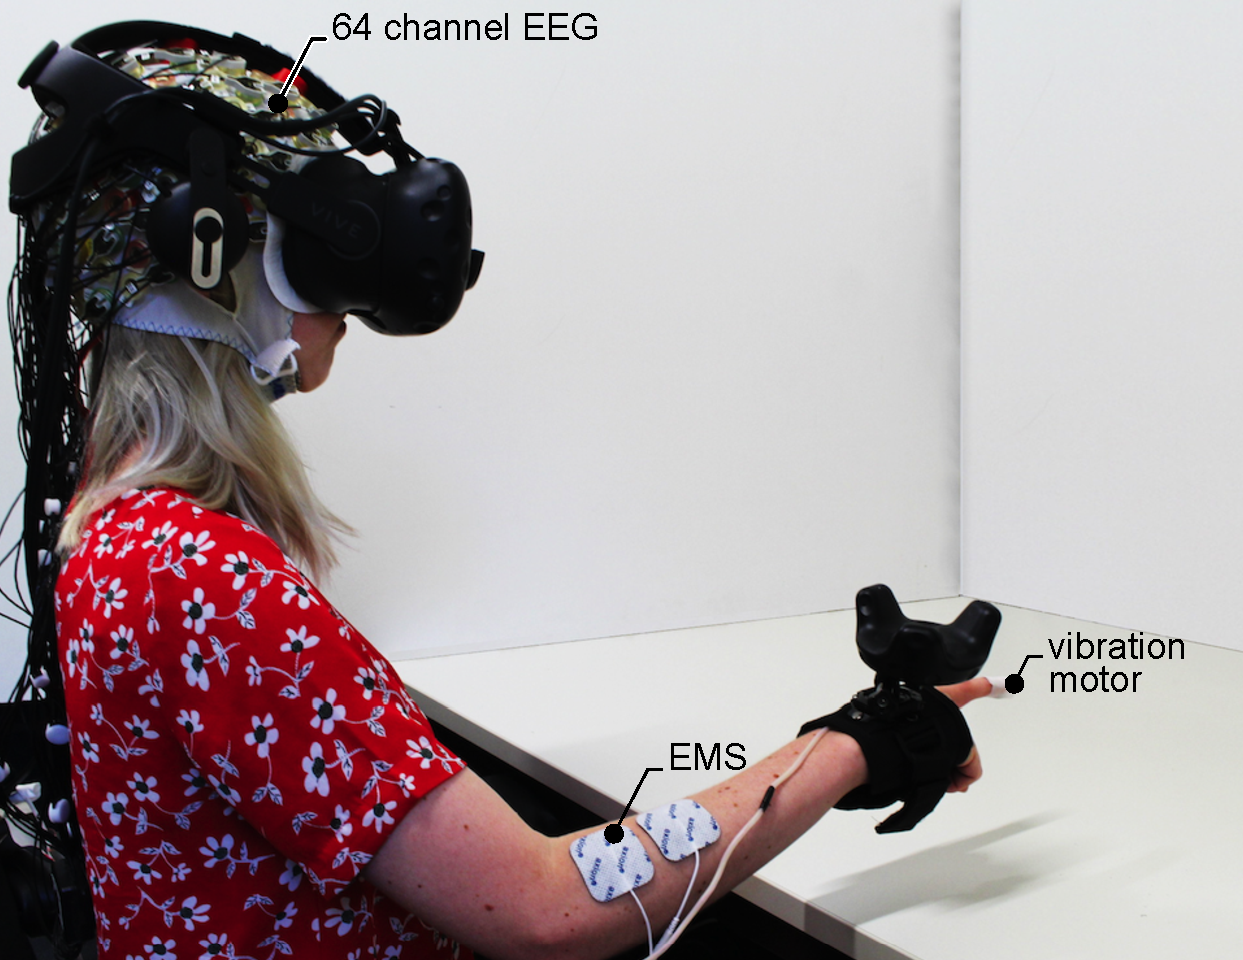
\includegraphics[width=\linewidth]{figures/experiment.pdf}
%\missingfigure[figcolor=white]{Shows setup.}
%\vspace{-17pt}
\caption{Our experimental setup (image with consent from participant).}
\label{setup}
\end{figure}

\textbf{(1) VR and hand tracking.} We used an HTC Vive headset (HTC Corporation, Taoyuan, Taiwan) with the Vive Deluxe Audio Strap and custem EEG cap spacers \footnote{https://grabcad.com/library/adapter-for-vr-eeg-setups-1} to ensure a good fit and less discomfort due to the EEG cap. We used a Vive Tracker, attached to the participant's wrist, to track their right hand. 

\textbf{(2) Vibrotactile feedback.} We used a vibration motor (Model \textit{308-100} from \textit{Precision Microdrives}), which generates 0.8g at 200Hz. This motor measures 8mm in diameter, making it ideal for the fingertip. The vibration feedback was driven at 70mA by a 2N7000 MOSFET, which was connected to an Arduino output pin at 3V.

\textbf{(3) Force feedback.} We actuated the index finger via electrical muscle stimulation (EMS), which was delivered via two electrodes attached to the participants' \textit{extensor digitorum} muscle. The finger actuation was achieved via a medically-compliant battery powered muscle stimulator (\textit{Rehastim} from \textit{Hasomed}), which provides a maximum of 100mA and is controllable via USB. 

% We utilized the extensor digitorum since we found that we can robustly actuate it without inducing parasitical motion of neighboring muscles; this was verified during pilot studies. This finger actuation was achieved via a medically-compliant battery powered muscle stimulator (\textit{Rehastim} from \textit{Hasomed}), which provides a maximum of 100mA and is controllable via USB. We chose this device since it had been successfully used by researchers as a means to generate force feedback in both VR~\cite{lopes_walls_2017} and AR~\cite{lopes_AR}. The EMS was pre-calibrated per participant to ensure a pain-free stimulation and robust actuation. 

\textbf{(4) EEG Setup.} EEG data was recorded from 64 actively amplified electrodes using BrainAmp DC amplifiers from BrainProducts. Electrodes were placed according to the extended 10\% system ~\cite{oostenveld_five_2001}. After fitting the cap, all electrodes were filled with conductive gel to ensure proper conductivity and electrode impedance was brought below 5kOhm for all electrodes. EEG data was recorded with a sampling rate of 1000 Hz. We synchronized tracking, EEG data, and an experiment marker stream that marked sections of the study procedure using labstreaminglayer\footnote{https://github.com/sccn/labstreaminglayer}.

\begin{figure*}[!ht]
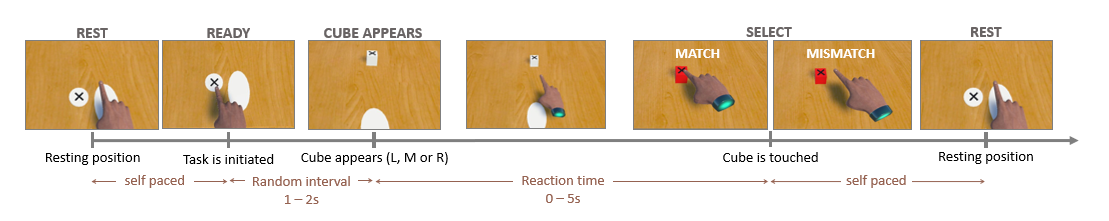
\includegraphics[width=\linewidth]{figures/Task_mismatch.PNG}
\vspace{-15pt}
\caption{Interaction flow depicting one trial in our 3D object selection task.}
\label{task_flow}
\end{figure*}

\subsection{Training phase}
We asked participants to wear the HTC VIVE VR headset for a maximum of 24 trials practice trials. Overall, the EEG fitting, calibration, and practice trials took around 30 minutes (with two experimenters).

\subsection{Task}
Participants performed a 3D object selection task in VR design with Unity Software (Unity Technologies, San Francisco, USA). The interaction flow of our task, depicted in Figure~\ref{task_flow}, was as follows: (1) participants moved their hands from the \textit{resting position} to the \textit{ready position}, to indicate they were ready to start the next trial; (2) participants waited for a new target to appear (the time of a new target spawning was randomized between 1-2 s); (3) then, the target (a cube) would appear in one of three possible positions (center, left, right), all equidistant from the participant's \textit{ready position}; (4) then, participants acquired the target by moving and touching the target with their index finger. (5) After a target was acquired, participants moved back to the \textit{resting position}. Here, they could take a break before the next trial.

\subsection{Interface conditions}
Participants performed the task in three additive feedback conditions:

(1) \textbf{visual-only (Visual)}: when participants touched the cube, it changed its color from white to red (visual feedback)
% ; our no-haptics \textbf{baseline}~\\
\indent(2) \textbf{tactile (Vibro)}: when participants touched the cube in the vibro condition, they received a 100 ms vibroactile stimulus and the color change (visual + tactile feedback)
% ; this is the only available haptic feedback in today's VR experiences.~\\
\indent(3) \textbf{force-feedback (EMS)}: in this condition, participants also received a 100 ms of EMS stimulation at the index finger extensor in addition to the visual and vibrotactile feedback (visual + tactile + force feedback)
% . As prior research showed the EMS stimulation of the opposing muscle (in our case, the extensor) is perceived as the resisting force that arises from pushing against the cube (i.e., force feedback)~\cite{lopes_muscle-propelled_2013,lopes_walls_2017,lopes_impacto:_2015}.

% We designed our three feedback conditions additively because additional haptic feedback is generally associated with more haptic realism, therefore, we hypothesized that ERPs would demonstrate some correlation to the ascending level of the feedback's realism.

\subsection{Introducing Visuo-Haptic Mismatches}
To allow us to compare the event-related EEG and movement signatures in a realistic vs. unrealistic interaction, we presented participants with two different classes of trials: \textbf{match trials (C)} (75\% of the trials) and \textbf{mismatch trials (M)} (25\%). This procedure elicits a prediction mismatch signal in 25\% of the trials similar to previous designs investigating the impact of target probabilities~\cite{polich_updating_2007}.  %on ERP modulations
In the \textbf{matching} trials, the feedback stimuli were presented upon touching the object, exactly when participants expected them to occur based on the available visual information (finger touching the target). In contrast, in the \textbf{mismatch} trials, the feedback stimuli were triggered prematurely, which was accomplished by enlarging the invisible radius of touch detection by 350\%. While in the match trials, we used a cube collider of the exact size of the VR cube, in the mismatch trials, we used a larger sphere collider. Our collider enlargement was based on the study design by Singh et al.~\cite{singh_visual_20008}, in which they showed that VR users can detect a visual mismatch at around 200\% of offset from the target. In our pilot tests, we decided to extend the offset to 350\% to make the mismatch more obvious so as to provoke more pronounced prediction errors. 

Also, we used a match-to-mismatch ratio of 75\%-25\% of the total trials by modeling our study after previous studies, which also ensure that participants are faced with a detectable unrealistic behavior of the virtual environment~\cite{Liao2011,Wiersema2007,Donchin1988}. For these unrealistic trials to occur, the participants must first be able create a stable model of how the VR world operates, thus the VR world cannot behave at a random 50\%-50\% match-mismatch ratio.

Finally, these match vs. mismatch trials were presented in five randomly generated sequences, each with an equal distribution of matches and mismatches.

\subsection{Experimental design}
The experiment consisted of five phases: (1) a setup phase; (2) a calibration phase; (3) a short training phase; (4) the task itself, in all three possible interface conditions, each followed by a subset of items from the IPQ questionnaire (G1, REAL2, SP4 and INV1)~\cite{T.W.Schubert2003} and the NASA-TLX~\cite{Hart1988}. Lastly (5) participants were asked about their experience in the VR and which condition they enjoyed the most.

% For completeness, at the end of each condition we presented the four most relevant questions from the standard IPQ~\cite{ipq_paper}, in particular: G1, REAL2, SP4 and INV1. However, our hypothesis was that the inclusion mismatch trials, which were presented in 25\% of the cases, would lower the IPQ ratings dramatically.

We used a within-subjects design with 300 trials for each, the Visual and Vibro feedback condition, and 100 trials for the EMS condition. The order of the Visual and Vibro conditions was randomized across participants with the EMS condition always being the last block. 
% This was done to avoid potential overshadowing of the EMS stimulation (a very strong sensation) on the two other stimulation conditions.





%%%%% resources:
% \subsection{Task and Procedure}
% Using an HTC Vive VR Headset with the Vive Deluxe Audio Strap and a Vive Tracker (HTC Corporation, Taoyuan, Taiwan) attached to the right hand, a 3D object selection task was presented on a virtual table placed on an infinite white plane. The virtual environment was created in the Unity3D engine (Version, company details). White cubes appeared at random either in the center, to the left, or to the right of the participant, equidistant from a starting position (see Figure ??). The time of a new cube spawning was randomized between 1-2 seconds after starting a trial. 

% %no subsections? This so hard to parse, make a task heading or so?
% Participants were tasked to select the cube with their index finger and, upon completion, move their hand back to a resting position indicated on the table. The task was completed in two blocks of 300 trials each, with one block providing visual-only feedback, i.e. the cube changing its color from white to red upon selecting, and one block providing visual-tactile feedback, in which the selection contact was indicated by the color change plus a small vibrotactile pulse. Placed under the index fingertip, a vibration motor (Model \textit{308-100} from \textit{Precision Microdrives}), generating 0.8g at 200Hz and measuring 8mm in diameter was driven at 70mA by a 2N7000 MOSFET connected to an Arduino output pin at 3V. An initial 24 trial training session was followed by the two experimental blocks (balanced across participants), each followed by two questionnaires, NASA-TLX and IPQ. For the main experimental manipulation of asynchrony, 25\% of the trials (totalling 75 asynchronous trials per feedback block of 300 trials) exhibited spatio-temporal asynchrony in line with established oddball paradigms. Object selection was triggered prematurely by bounding a spherical collider to the cube and enlarging it by 350\% in comparison to a collider bounded to the shape of the cube in the synchronous trials. Asynchronous trials were sorted in a pseudo-randomized sequence following synchronous trials, i.e. between one and five synchronous trials preceeded an asynchronous trial. Extended task and apparatus descriptions can be found elsewhere \cite{Gehrke2019}.
% % todo add movie, figure and references